\documentclass{standalone}
\usepackage{preset}
\begin{document}
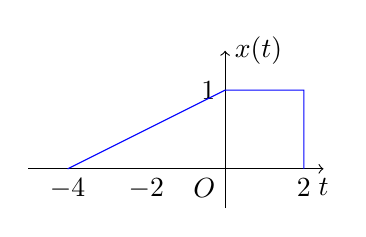
\begin{tikzpicture}[x=5mm,y=10mm]
    \draw[->](-5,0)--(2.5,0)node[below]{\(t\)};
    \draw[->](0,-.5)--(0,1.5)node[right]{\(x(t)\)};
    \draw(0,0)node[below left]{\(O\)};
    \foreach \x in {-4,-2,2}{
        \draw(\x,0)node[below]{\(\x\)};
    }
    \draw(0,1)node[left]{\(1\)};
    \draw[blue](-4,0)--(0,1)--(2,1)--(2,0);
\end{tikzpicture}
\end{document}
